%!TEX root = ../thesis.tex

\thispagestyle{myheadings}

\graphicspath{{Body/Figures/RatioAnalysis/}{Body/Figures/RatioAnalysis/MethodOverview/}}

\chapter{\texorpdfstring{\wa}{wa} Measurement}
\label{chapter:SpinPrecessionMeasurement}




The measurement of \wa is determined by counting the number of detected positrons in the calorimeters above some energy threshold, as described in \secref{section:WaIntro}. The calorimeters measure hit times and energies of impacting particles, where these hit times and energies are determined from SiPM current signals and reconstructed



\section{Reconstruction}
\label{sec:ReconWest}



-two reconstructions which are useful to compare, but I use reconwest
-GPUs used to do online processing before any data is saved





-overview of reconstruction

-need to mention gain


-clustering


The reconstruciont process is described in detail by A. Fienberg \cite{AFThesis}



\section{Histogramming}
\label{sec:Histogramming}


-artificial deadtime
-time randomization

-here or maybe in a later section mention the pileup procedure, maybe a subsection


\section{Lost muons}
\label{sec:lostmuons}

\section{Fitting}
\label{sec:Fitting}


-detail the ratio method - might need to pull stuff out from my appendix


    \begin{figure}[]
    \centering
        \begin{subfigure}[t]{0.45\textwidth}
            \centering
            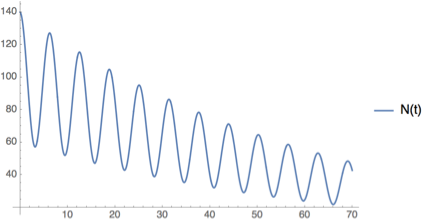
\includegraphics[width=\textwidth]{FiveParamFunc}
            \caption{}
        \end{subfigure}%

        \vspace{2mm}
        \begin{subfigure}[t]{0.45\textwidth}
            \centering
            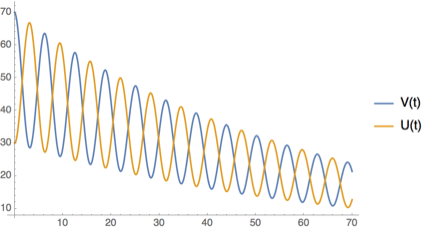
\includegraphics[width=\textwidth]{UVFuncs}
            \caption{}
        \end{subfigure}
        \begin{subfigure}[t]{0.45\textwidth}
            \centering
            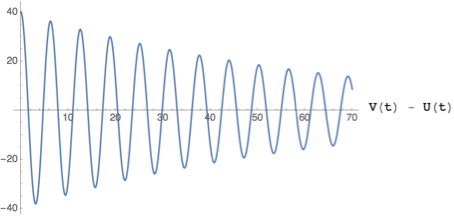
\includegraphics[width=\textwidth]{RatioNumFunc}
            \caption{}
        \end{subfigure}%
        \vspace{2mm}
        \begin{subfigure}[t]{0.45\textwidth}
            \centering
            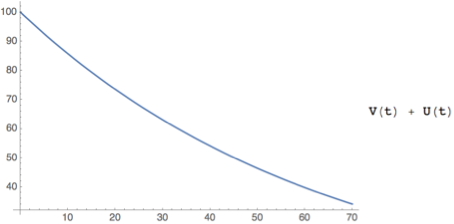
\includegraphics[width=\textwidth]{RatioDenomFunc}
            \caption{}
        \end{subfigure}
        \begin{subfigure}[t]{0.45\textwidth}
            \centering
            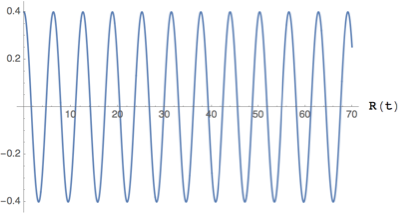
\includegraphics[width=\textwidth]{RatioFunc}
            \caption{}
        \end{subfigure}% 
    \caption[]{}
    \label{}
    \end{figure}






\section{Systematic errors}
\label{sec:Systematic Errors}



\cleardoublepage
